
\section{Metrics Collection}
\label{sec:metrics_collection}

During each benchmark run, the Workload Generator submits synthetic transactions according to the configured workload profile. For steady-state experiments, the workload follows a Poisson-style arrival process to approximate independent transaction arrivals. Each RollupX component records telemetry locally inside its container, and the benchmark scripts export the collected measurements as JSON, JSONL, and CSV files under \path{benchmark-suite/metrics/}. These raw files are later processed by the aggregation pipeline to produce run-level performance and cost summaries.

Table~\ref{tab:metric_definitions} defines the main metrics used in the evaluation. The metrics are selected to capture both user-facing performance, such as throughput and latency, and system-facing overheads, such as data availability footprint and Layer-1 submission cost.

\begin{table}[!htbp]
\centering
\caption{Metric Definitions}
\label{tab:metric_definitions}
\small
\setlength{\tabcolsep}{4pt}
\renewcommand{\arraystretch}{1.15}
\begin{tabularx}{\textwidth}{@{}p{0.24\textwidth}p{0.16\textwidth}X@{}}
\toprule
\textbf{Metric} & \textbf{Unit} & \textbf{Definition / Measurement Source} \\
\midrule

Throughput
& TPS
& Measures the rate of successfully processed transactions. Submitted throughput is derived from the Workload Generator, while committed throughput is computed from transactions included in batches submitted to Layer 1. \\

\addlinespace

Latency
& Seconds / milliseconds
& Measures the time from transaction submission to soft finality, where soft finality refers to inclusion in a sealed Layer-2 batch. Average, P95, and P99 latency values are used where available. \\

\addlinespace

Finalization time
& Seconds
& Measures the time from batch sealing to hard finality, where hard finality refers to confirmation of the corresponding Layer-1 submission transaction. \\

\addlinespace

Proof time
& Seconds / milliseconds
& Measures the time spent in the proving stage. For mock prover experiments, this reflects the configured proof delay. For real prover experiments, it captures the observed prover execution time. \\

\addlinespace

Cost per transaction
& Gas / Wei
& Measures the total Layer-1 submission cost for a batch divided by the number of transactions in that batch. This includes regular gas cost and blob-related cost when applicable. \\

\addlinespace

Data availability footprint
& Bytes
& Measures the size of the encoded, compressed, or blob-formatted batch payload submitted or committed through the selected data availability mode. \\

\bottomrule
\end{tabularx}
\normalsize
\end{table}

The telemetry pipeline used to collect and aggregate these measurements is shown in Figure~\ref{fig:metrics_telemetry_pipeline}. The pipeline separates component-level metric generation from post-run aggregation, allowing the benchmark suite to preserve raw logs while also producing summarized tables and plots for analysis.

\begin{figure}[!htbp]
    \centering
    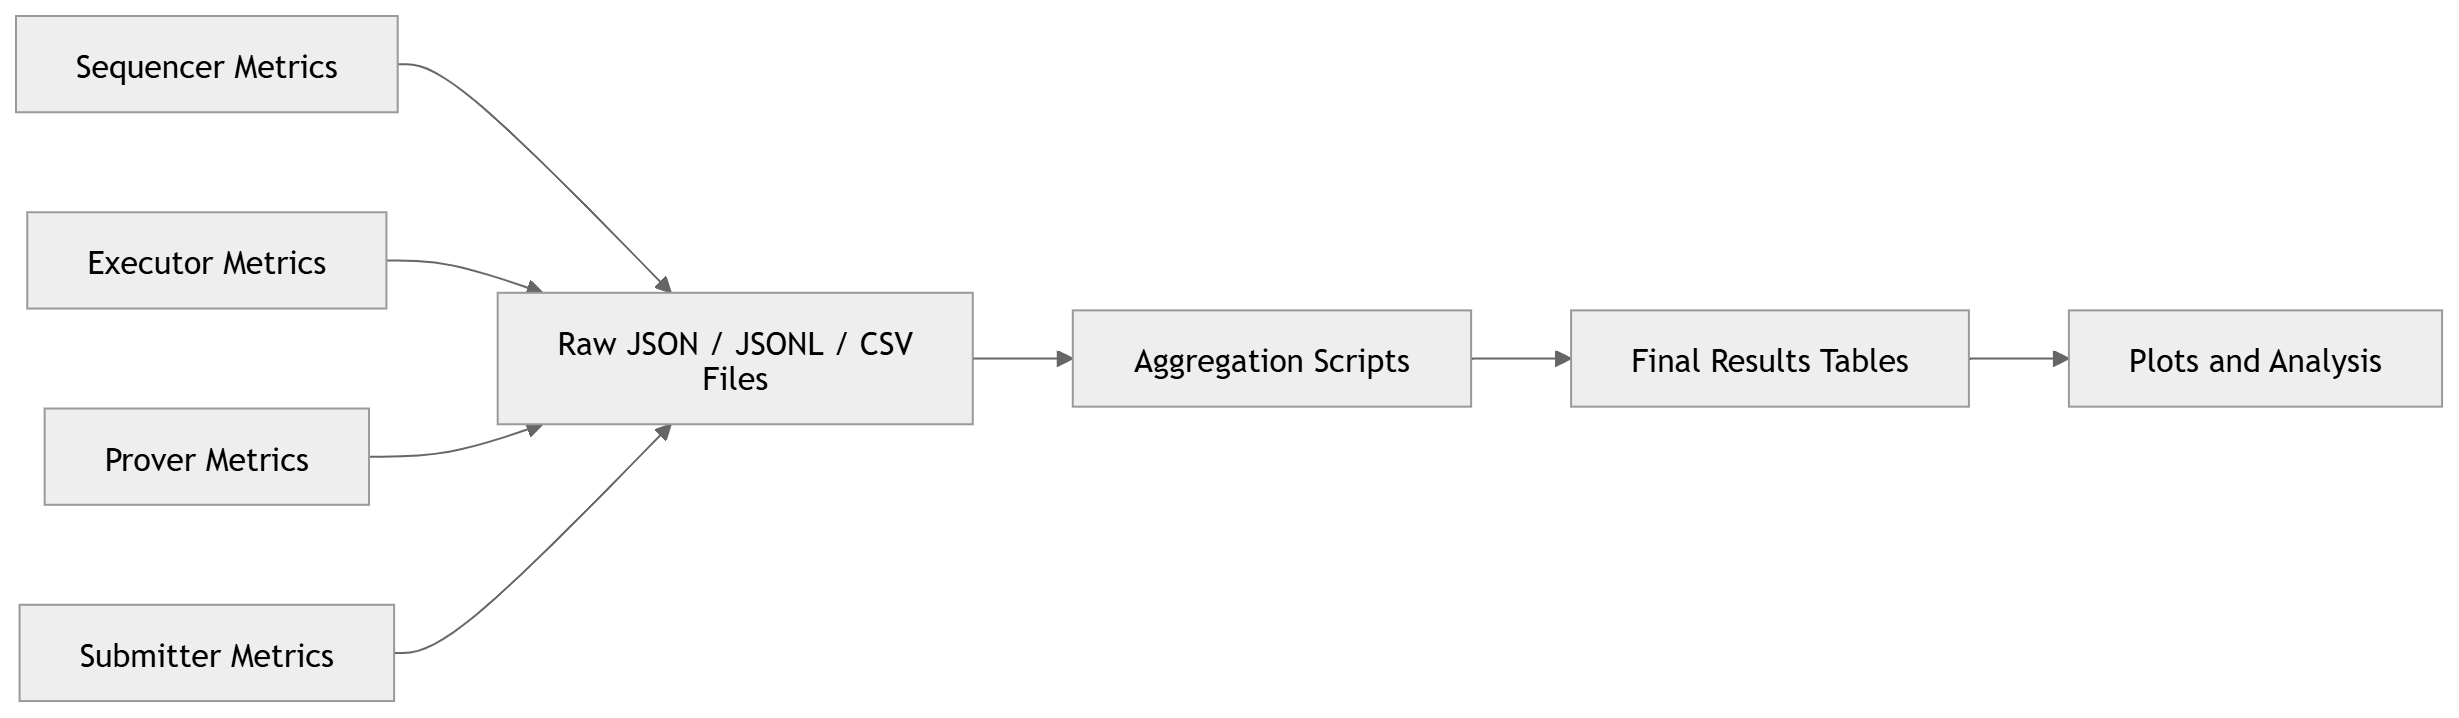
\includegraphics[
        width=0.92\textwidth,
        keepaspectratio
    ]{figures/chapter5/metrics_telemetry_pipeline.png}
    \caption{Metrics and telemetry pipeline used for benchmark aggregation.}
    \label{fig:metrics_telemetry_pipeline}
\end{figure}

Figure~\ref{fig:metrics_telemetry_pipeline} summarizes how telemetry flows through the benchmark suite. The Sequencer records queueing, batching, sealing, and policy-related measurements. The Executor records batch execution and state-transition measurements. The Prover records proof-delay or proof-execution measurements, depending on the configured prover mode. The Submitter records payload size, data availability mode, Layer-1 gas usage, transaction receipt information, and finalization latency.

After each benchmark run, the raw metric files are processed by the aggregation scripts to generate final result tables and plots. These outputs are then used to analyze throughput, latency, proving overhead, data availability footprint, and Layer-1 cost across different benchmark configurations.

